\section{Gym Vouchers}
\begin{minipage}[t]{0.5\textwidth}
    The school gym operates commercially, which means it charges fees. However, the WeChat mini-program “XJTLU Sports Center” distributes vouchers worth 100 yuan every month. These can be used for booking basketball courts, table tennis tables, gym time, etc. For more details, please explore the mini-program. In fact, the school’s gym facilities are very comprehensive and quite new. If you haven’t been there yet, go explore it soon. The vouchers are essentially [expiring balance], which means they will automatically adjust. For example, if you book a gym session for 25 yuan using a 100 yuan voucher, the voucher balance will become 75 yuan, but the vouchers do have an expiration date.

    After booking, you need to swipe your XJTLU campus card to enter the gym’s main entrance, and then scan the QR code of the booked facility to enter the specific venue.

    \begin{flushright}
    (October 12, 2022 by \Wu) \\
    (Translated by GPT)
    \end{flushright}
\end{minipage}
\begin{minipage}[t]{0.45\textwidth}
    \begin{figure}[H]
        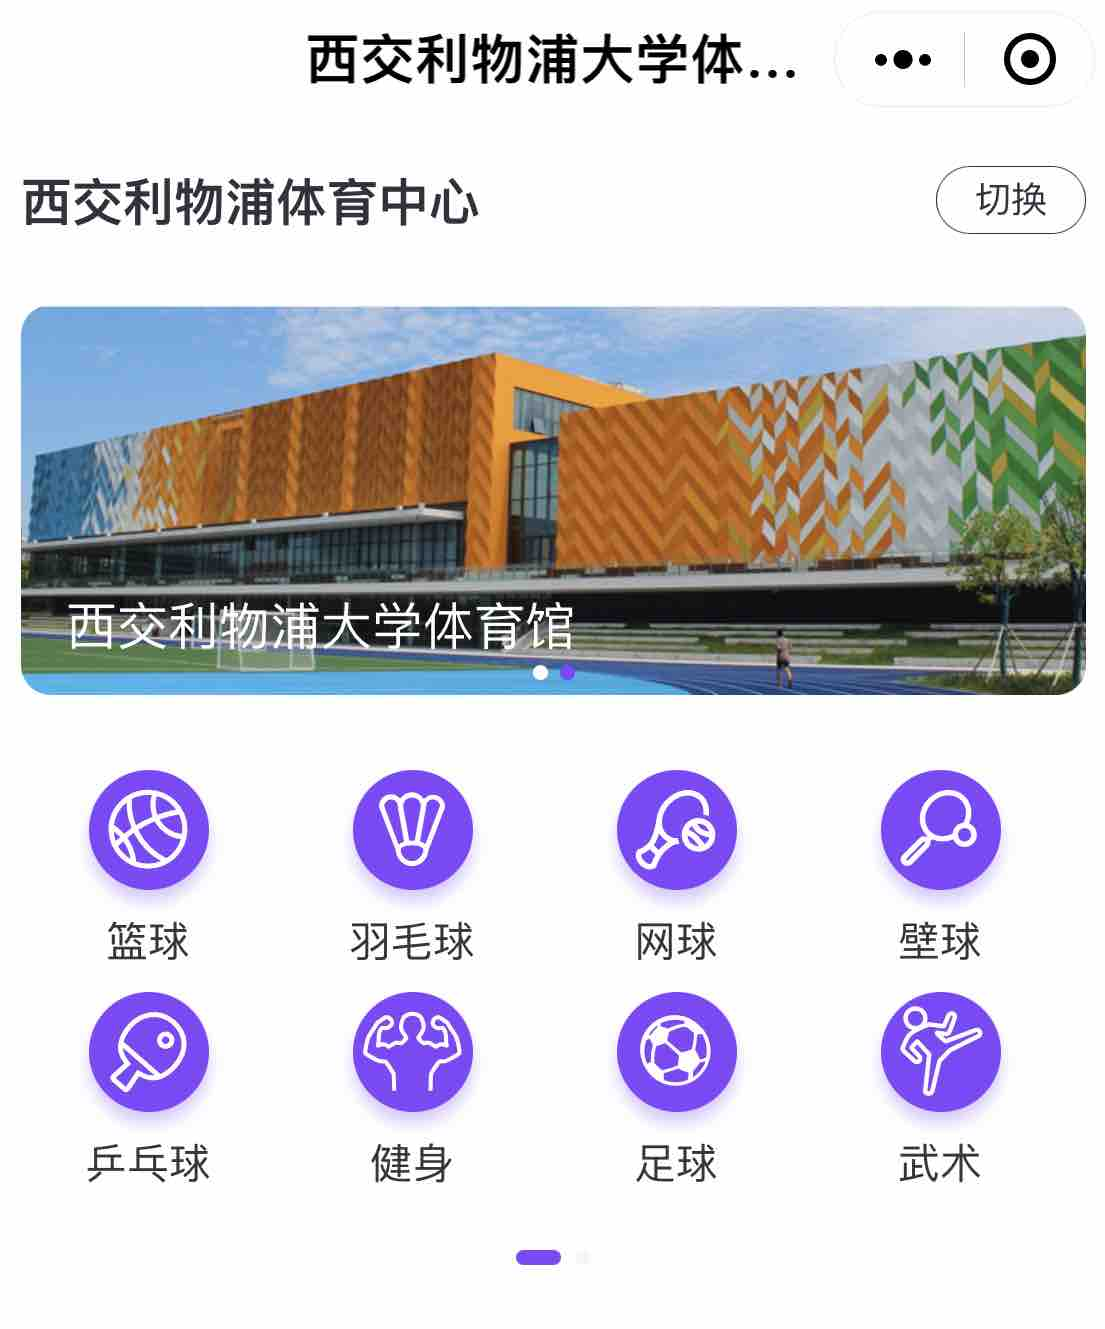
\includegraphics[width=0.95\columnwidth, right]{author-folder/Kai.Wu/sportcenter_miniprogram.jpg}
    \end{figure}
\end{minipage}
